\documentclass[letterpaper, 12pt]{article}
\title{CSE471 - Homework 7}
\author{Kumal Patel}
\date{\today}

\usepackage{amsmath, float, graphicx}
\begin{document}
\maketitle

\begin{enumerate}
    \item[1.1]
        \begin{enumerate}
            \item
                  \begin{gather*}
                      (x_1-a)^2+(x_2+b)^2-r^2=0 \\
                      x_1^2-2ax_1+x_2^2-2bx_2+a^2+b^2-r^2 = 0\\
                      -2ax_1-2bx_2+x_1^2+x_2^2+(a^2+b^2-r^2) = 0
                  \end{gather*}
                  By mapping this to the feature space you get $w_1=(-2,-2,1,1)$
                  and intercepts of $a^2+b^2-r^2$. And circular boundary lies
                  linear to feature space which allows for linear separability.
            \item
                  \begin{gather*}
                      c(x_1-a)^2+d(x_2-b)^2-1=0 \\
                      cx_1^2-2acx_1+dx_2^2-2bdx_2+a^2c+b^2d-1=0 \\
                      -2acx_1-2bdx_2+cx_1^2+dx_2^2+(a^2c+b^2d-1)=0
                  \end{gather*}
                  By mapping this to the feature space you get $w_1=(-2ac,-2bd,c,d,0)$
                  and intercepts of $a^2c+b^2d-1$. And circular boundary lies linear to
                  feature space which allows for linear separability.
        \end{enumerate}
    \item[1.2]
        \begin{enumerate}
            \item
                  \begin{gather*}
                      \pi^p(1-\pi)^n
                  \end{gather*}
            \item
                  \begin{gather*}
                      L = plog(\pi) + nlog(1-\pi) \\
                      \frac{\partial L}{\partial \pi}= \frac{p}{\pi}-\frac{n}{1-\pi}=0 \\
                      p(1-\pi) - n\pi = 0 \\
                      p-p\pi-n\pi = 0 \\
                      p = p\pi+n\pi \\
                      p = \pi(p+n) \\
                      \pi = \frac{p}{p+n}
                  \end{gather*}
            \item .
                  \begin{figure}[H]
                      \centering
                      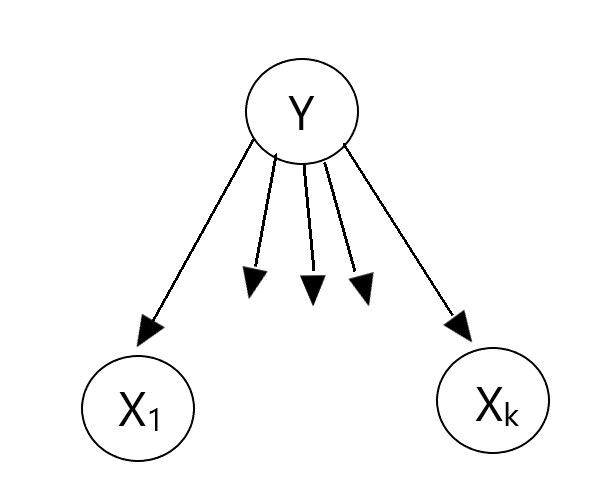
\includegraphics[width=0.5\linewidth]{q2_c.png}
                      \caption{Bayesian Network of such assumption }
                  \end{figure}
            \item
            \item

        \end{enumerate}
    \item[1.3]
        \begin{enumerate}
            \item
                  \begin{gather*}
                      P(Y=spam | w_1 = perfect, w_2 = self) P(Y = spam)> P(Y = ham | w_1 = perfect, w_2 = self) P(Y=ham)\\
                      1/8 * 1/4 * P(Y=spam) > 1/12 * 1/4 * (1- P(Y=spam)) \\
                      1/32 * P(Y=spam) > 1/48 * (1-P(Y=spam)) \\
                      1/32 * P(Y=spam) > 1/48  - 1/48 * P(Y=spam) \\
                      3/96 * P(Y=spam) > 2/96  - 2/96 * P(Y=spam) \\
                      5/96 * P(Y=spam) > 2/96 \\
                      P(Y=spam) > 2 / 5
                  \end{gather*}
            \item
                  There are two methods of determining if an email is spam, one using bag-of-words model, and two using a
                  dictionary model. Bag-of-words model returns the number of occurrences of a specific word. And a dictionary
                  model returns if the specific word exists in the email. So for an email like 'Word count, word list, word dict',
                  where 'word' is the specific word we are searching for. Bag-of-words model will return 3 because there are 3 occurrences
                  of 'word', and dictionary will return 1 because 'word' exists in that email. Because bag-of-words model would return
                  a higher weight than dictionary model it is a better method to determine spam. Because one occurrence is not good as a
                  generic word like 'word' can be used without being spam. So the higher weight will determine spam.
            \item Bag-of-words model
                  \begin{gather*}
                      P(W=Dear | Y = spam) = 1/16 \\
                      P(W=lunch | Y = ham) = 1/9 \\
                      P(W=ASU | Y = ham) = 0
                  \end{gather*}
            \item Dictionary Model
                  \begin{gather*}
                      P(W=Dear | Y = spam) = 1/2 \\
                      P(W=lunch | Y = ham) = 1/2 \\
                      P(W=ASU | Y = ham) = 0
                  \end{gather*}
        \end{enumerate}
    \item[1.4]


\end{enumerate}


\end{document}